\documentclass[border=10pt]{standalone}
\usepackage{pgfplots}
\usepgfplotslibrary{groupplots}
\pgfplotsset{compat=1.18}
\begin{document}
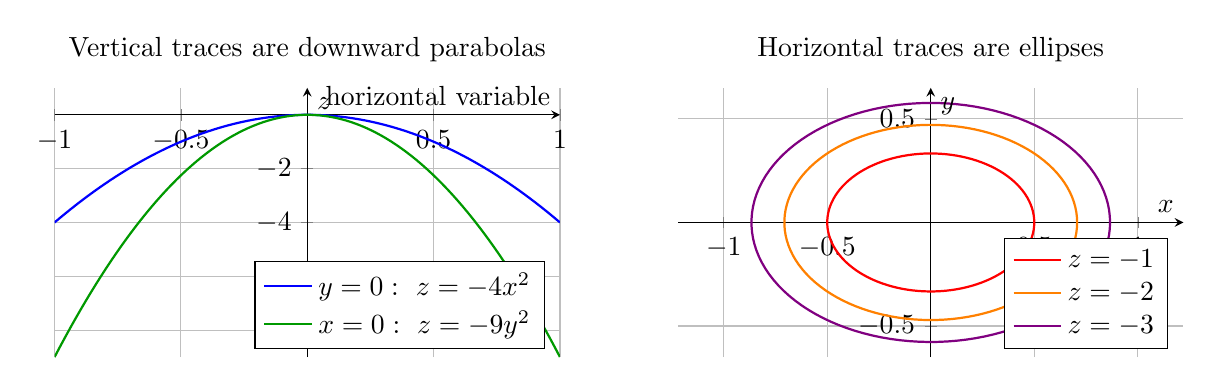
\begin{tikzpicture}
\begin{groupplot}[
  group style={group size=2 by 1, horizontal sep=1.5cm},
  width=8cm, height=5cm,
  axis lines=middle,
  grid=major,
  enlargelimits=false
]
\nextgroupplot[
  xlabel={horizontal variable},
  ylabel={$z$},
  title={Vertical traces are downward parabolas},
  legend pos=south east,
  xmin=-1, xmax=1,
  ymin=-9, ymax=1
]
\addplot[blue, thick, domain=-1:1, samples=100] {-4*x^2};
\addlegendentry{$y=0:\ z=-4x^2$}
\addplot[green!60!black, thick, domain=-1:1, samples=100] {-9*x^2};
\addlegendentry{$x=0:\ z=-9y^2$}

\nextgroupplot[
  xlabel={$x$},
  ylabel={$y$},
  title={Horizontal traces are ellipses},
  axis equal,
  xmin=-0.9, xmax=0.9,
  ymin=-0.65, ymax=0.65,
  legend pos=south east
]
\addplot[red, thick, domain=0:360, samples=120] ({sqrt(1/4)*cos(x)},{sqrt(1/9)*sin(x)});
\addlegendentry{$z=-1$}
\addplot[orange, thick, domain=0:360, samples=120] ({sqrt(2/4)*cos(x)},{sqrt(2/9)*sin(x)});
\addlegendentry{$z=-2$}
\addplot[violet, thick, domain=0:360, samples=120] ({sqrt(3/4)*cos(x)},{sqrt(3/9)*sin(x)});
\addlegendentry{$z=-3$}
\end{groupplot}
\end{tikzpicture}
\end{document}